\section{Results}
\label{sec:results}

We display the majesty of Moosinesq convection in Fig.~\ref{fig:dynamics}.
We visualize the temperature field $T$, so red is warm fluid that buoyantly rises, and blue is cold fluid that buoyantly falls.
Plotted over the temperature field is the mask $\mathcal{M}$, which is fully transparent when it is zero and which is a low-opacity white when $\mathcal{M} = 1$.
This allows us to show that, indeed, there are no appreciable motions outside of the moose and the mask is working properly.

The moose is filled with interesting dynamics\footnote{Likely due to a recent, delicious meal.}.
The legs largely serve as thin, tall ``tunnels'' which are filled with Von K\'{a}rm\'{a}n vortices and which connect the hot moose feet to its neutrally-buoyant body.
Cold fluid parcels from the body have managed to mix down one leg, and the moose would probably benefit from having that leg wrapped in a warm cloth or heat pack.
The body of the moose exhibits dynamics familiar from classical 2D Rayleigh-B\`{e}nard convection.
Hot and cold fluid swirl together, forming many vortices which eventually mix.
Aside from the legs, the antlers are the most interesting part of the moose.
Vortices of relatively hot fluid establish themselves there and remain for a few convective overturn times.
Then, violent flows from the moose's body disrupt those vortices with fresh, hot fluid and this process repeats itself.
Occasionally some of this hot fluid rises into the tips of the moose’s paddles, which explains how moose grow antlers.

\begin{figure*}[tp!]
\centering
    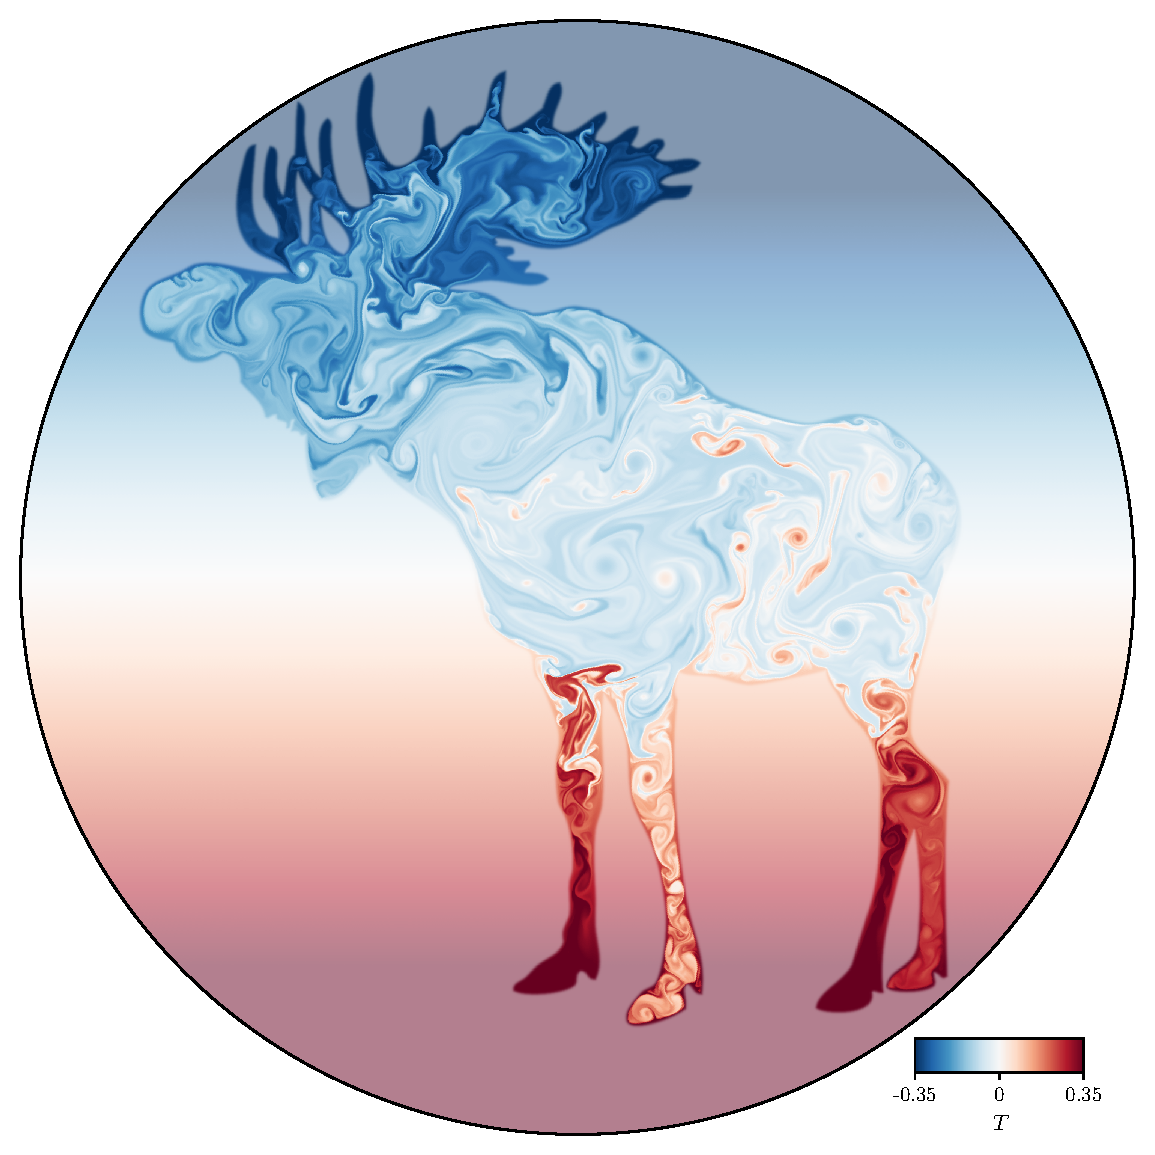
\includegraphics[width=\textwidth]{paper_figure02.pdf}
\caption{ 
    Here we visualize the temperature field in our simulation, where red is hot and buoyantly rises while blue is cold and buoyantly falls.
    We furthermore overplot the mask $\mathcal{M}$ on top of the temperature field in white with a low opacity; this does not affect the flow visualization within the moose but makes the region outside of the moose appear lighter in color.
    We do this to demonstrate that indeed, the flows are restricted to the area within $\mathcal{M}$ and therefore within the moose, as we expected.
    We encourage the reader to particularly note the beauty and power of the moose.
    An animated version of this figure is available online at \url{https://vimeo.com/693614276}.
    An animated version of the vorticity field in the same simulation can be found at \url{https://vimeo.com/693614600}.
\label{fig:dynamics}
}
\end{figure*}

Now that we have examined the dynamics in Moosinesq convection in some detail, we turn our attention towards its astrophysical applications.
\citet{kaiser_etal_2020} note that ``massive [sic] stars'' are sensitive to ``the details of their complex convective history''.
We agree.
When considering convective uncertainties in \emph{moosive} stars, previous authors have ignored the complex dynamics displayed in Fig.~\ref{fig:moosive_stars}.
That is, the cores of these stars are filled with Moosinesq convection, which can have important consequences for moosive stellar evolution.
It is unclear at this time how the complex flow morphologies associated with Moosinesq convection would affect e.g., the moosnetic fields, moosive stellar tracks, or lifetimes of these stars, nor do we measure the Van't Hoof factor \citep{vantHoof} to understand how Moosinesq convection affects the stellar chemical abundance profile.
We leave these important considerations to future work.

\begin{figure*}[t!]
\centering
    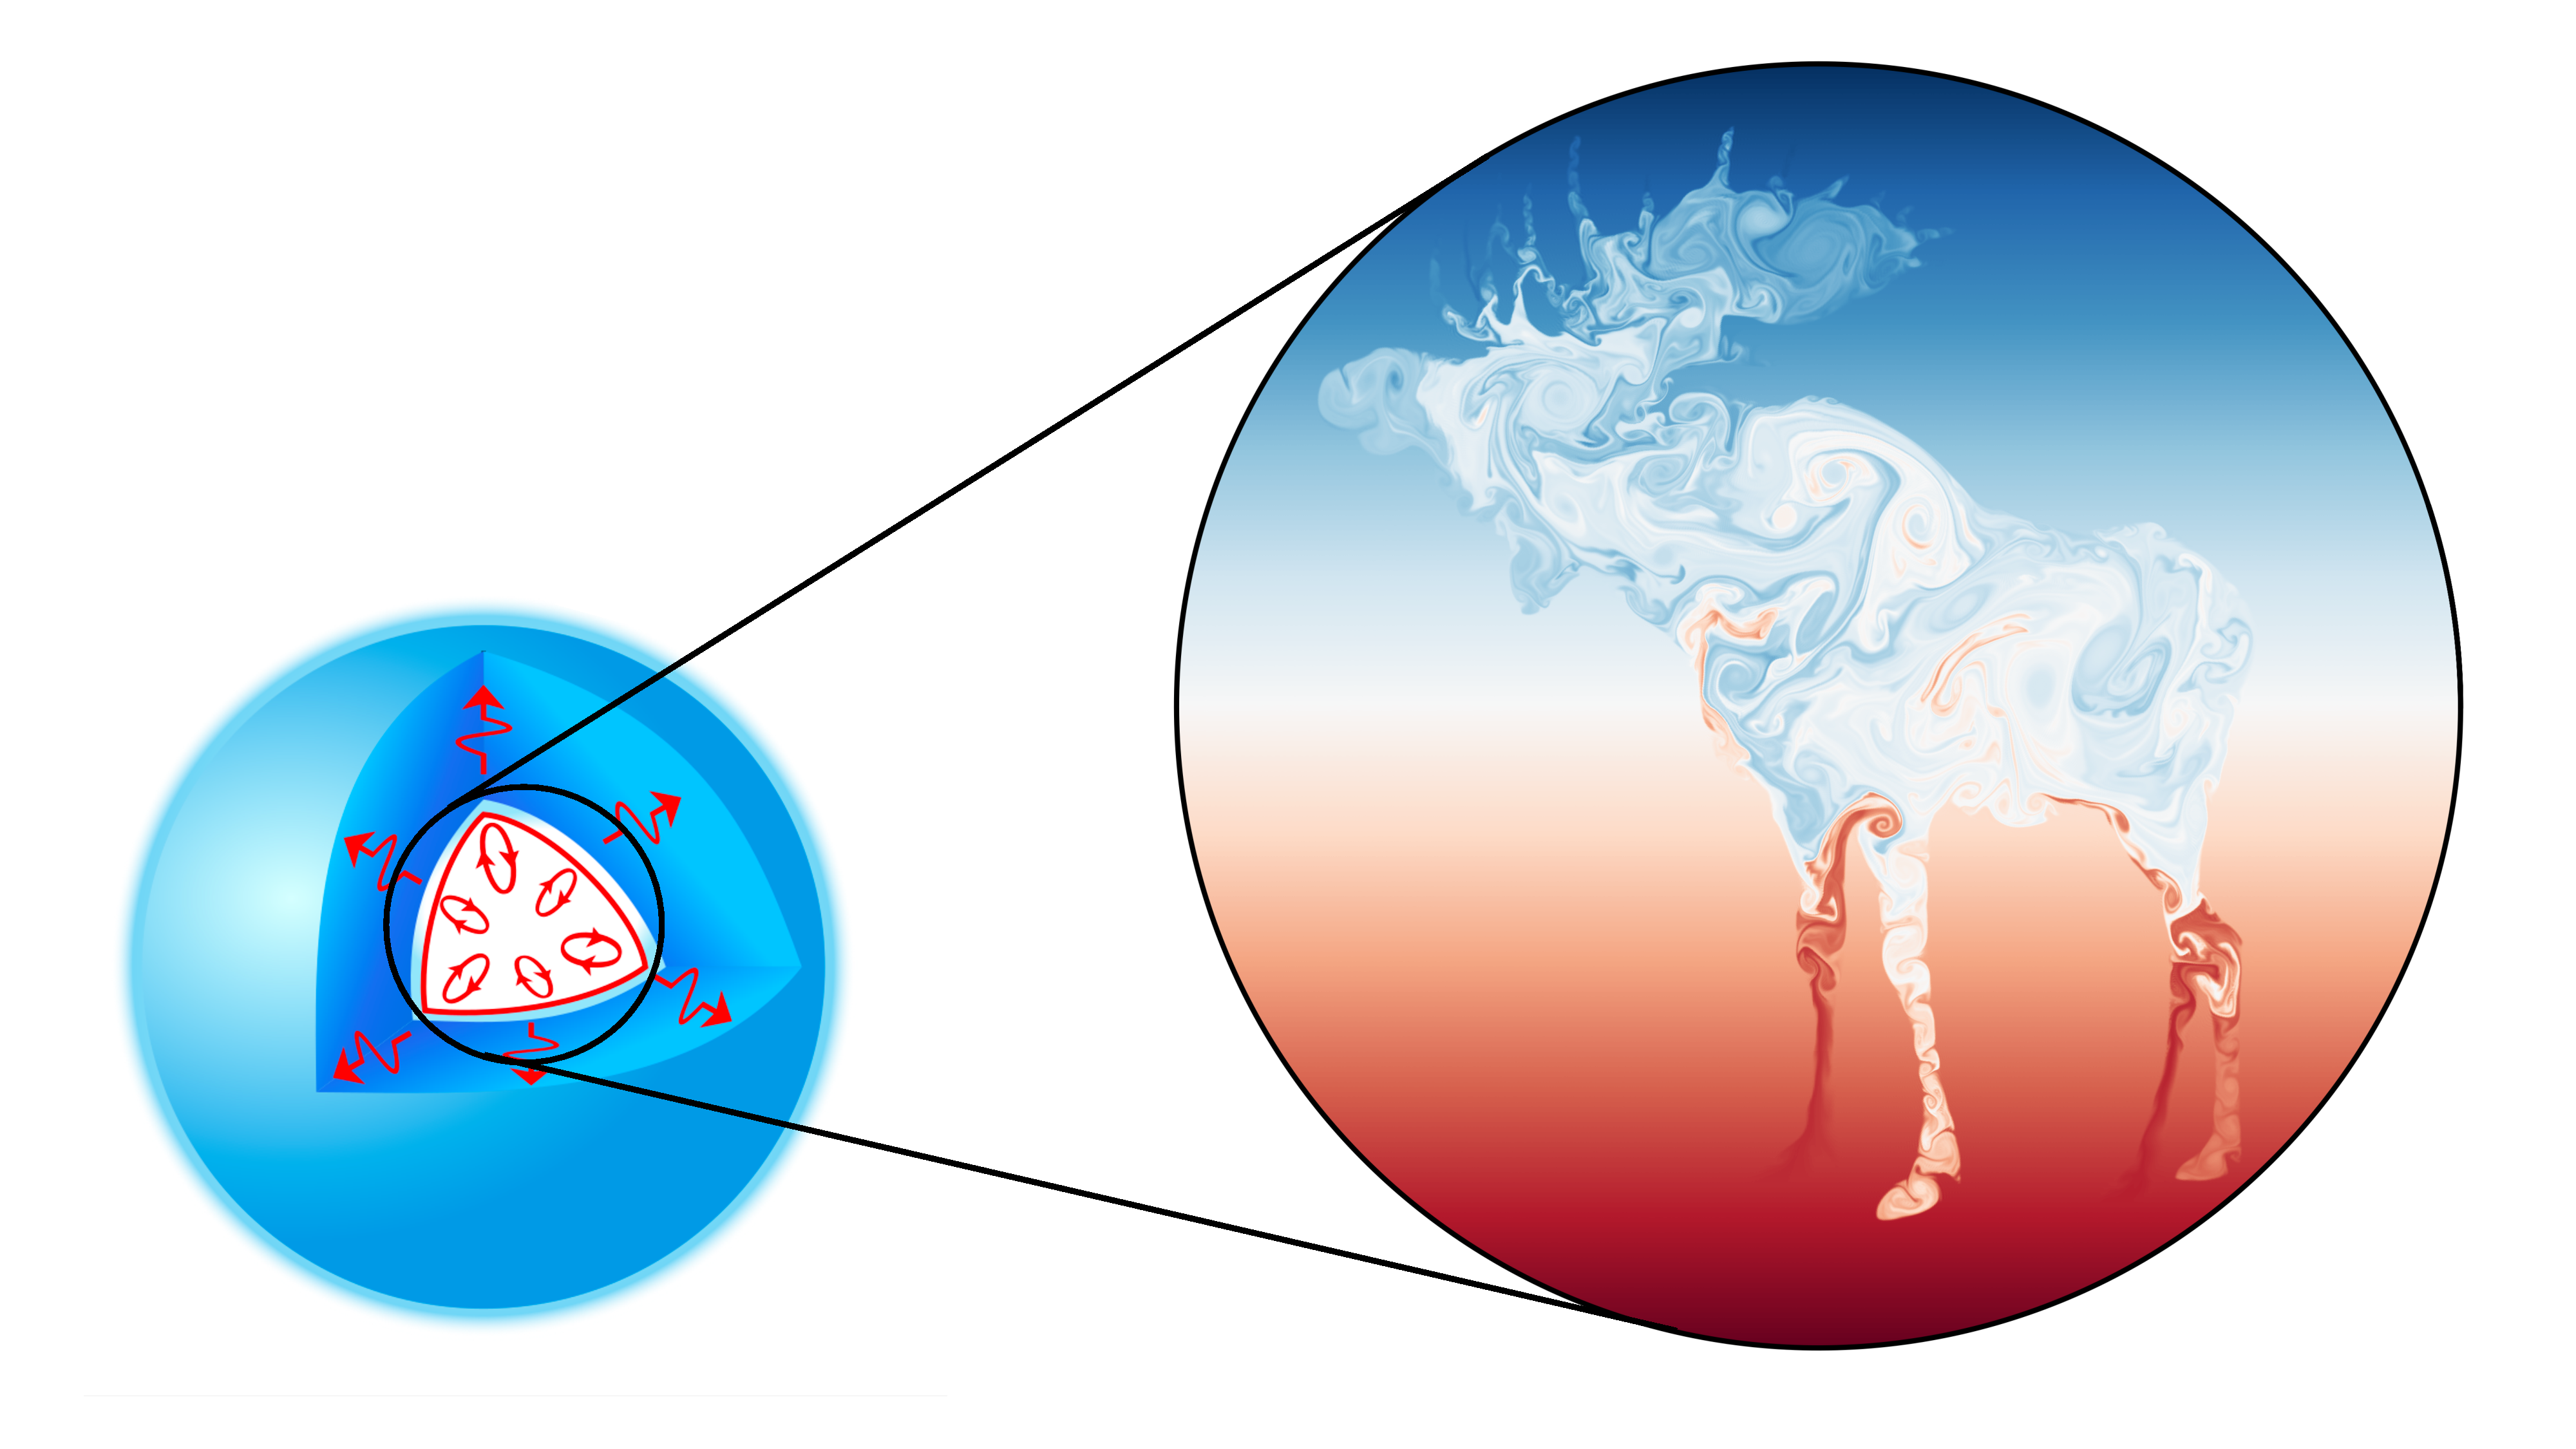
\includegraphics[width=\textwidth]{moosive_stars.pdf}
\caption{
    (Left) A diagram of a moosive star (source: \url{https://en.wikipedia.org/wiki/Stellar_structure}).
    (Right) The temperature field present in Moosinesq convection.
    We plot a circle around the core of the moosive star; we also plot some lines that lead to the circle around the Moosinesq convection simulation domain.
    This suggests that this convection is likely found within the core of these stars, but making this figure has increased our confusion as much as yours.
\label{fig:moosive_stars}
}
\end{figure*}


